\documentclass[11pt]{ctexart}
\usepackage[margin=1in]{geometry}
\usepackage{amsmath}
\usepackage{booktabs}
\usepackage{graphicx}
\usepackage{natbib}
\usepackage[colorlinks=true, linkcolor=blue, citecolor=blue, urlcolor=blue]{hyperref}

\graphicspath{{output/}{../output/}}

\title{数字化转型与企业生产率：一个合成数据经济学科研工作流示范}
\author{陈志远，中国人民大学商学院}
\date{2026年6月}

\begin{document}
\maketitle

\begin{abstract}
本文使用合成企业面板数据展示一个从实证估计、理论机制到正式写作的经济学研究工作流。实证部分采用双重差分设计，估计数字化转型状态与企业对数全要素生产率之间的关系；理论部分使用 Matlab 构造企业 AI 采用的成本收益优化模型，说明管理能力和采用成本如何影响企业采用 AI 的强度与生产率收益。所有数据均为模拟生成，本文结果仅用于教学和工作流演示，不能解释为真实企业数字化转型的因果证据。该工作流展示了如何将 Stata、Matlab、Jupyter notebook 和 \LaTeX{} 结合起来，形成可复现的科研写作流程。



\end{abstract}

\noindent\textbf{关键词：} 数字化转型；企业生产率；双重差分；事件研究；AI 采用；合成数据

\section{引言}
\subsection{背景与动机}

数字化转型是影响企业的重要决策，信息技术、自动化
和人工智能应用正在改变企业组织生产、处理信息和配置资源的方式。对经济学研究者而言，一个自然问题是：采用数字技术的企业是否在采用后表现出更高的生产率？更进一步，企业是否会因为采用成本和管理能力差异而做出不同的技术采用决策？本文围绕这些问题构造一个可复现的教学示范。示范的核心不是提供真实世界的估计结论，而是展示如何把 Stata 中的双重差分估计、Matlab 中的机制模型、Jupyter notebook 中的结果汇总和 \LaTeX{} 中的正式写作连接起来。

本文的研究对象是一个合成企业面板。处理组企业从 2020 年开始进入数字化转型状态，对照组企业没有进入该状态。实证模型控制企业固定效应和年份固定效应，并将标准误聚类到企业层面。主要估计结果显示，数字化转型状态与企业对数生产率之间的相关 DID 系数约为 0.1209，企业层面聚类标准误约为 0.0047。由于数据是人为构造的，这个数值只用于检查工作流是否能把分析结果传递到论文写作环节。



\section{文献综述}

本文的示范连接了两类文献。第一类文献讨论信息技术、自动化和人工智能对生产率与劳动市场的影响。\citet{BloomSadunVanReenen2012} 研究跨国企业的信息技术使用与生产率差异，强调管理和组织因素在 IT 收益中的作用。\citet{AcemogluRestrepo2019} 讨论自动化对任务结构的替代与创造，\citet{AgrawalGansGoldfarb2019} 则从预测成本下降的角度理解人工智能的经济影响。本文的 Matlab 模型沿用这一思路，将 AI 采用看作企业在生产率收益和实施成本之间的权衡。

第二类文献关注双重差分和事件研究方法。\citet{BertrandDufloMullainathan2004} 指出 DID 推断中序列相关和标准误处理的重要性，因此本文将标准误聚类到企业层面。对于多期处理和动态效应设定，\citet{CallawaySantAnna2021}、\citet{SunAbraham2021} 和 \citet{GoodmanBacon2021} 提醒研究者注意处理时点异质性和事件研究解释。本文的事件研究图只是合成数据中的识别诊断示范，不构成真实研究中的识别证明。

总体而言，现有研究共同表明：技术进步对生产率的作用取决于组织管理、任务重组与采用成本结构，经验识别策略与机制建模需要结合使用，才能更完整地理解企业数字化转型的经济后果。


\section{数据与变量}

合成数据覆盖 2016 至 2024 年的企业面板。核心结果变量为企业对数全要素生产率 $\log(TFP_{it})$。核心解释变量 $Digital_{it}$ 表示企业是否已经进入数字化转型状态。控制变量包括资本强度、出口份额和所有制变量。处理组企业在 2020 年后进入数字化转型状态，因此该变量同时包含处理组身份和处理后时期信息。

再次强调，样本并不来自真实企业数据库。数据生成过程被设计为服务于现场演示：一方面，它要足够接近经济学论文的分析流程；另一方面，它必须可被 Python、Stata、Matlab、Jupyter 和 \LaTeX{} 共同读取和复现。

表 \ref{tab:descriptives} 报告核心变量的描述统计。\texttt{log\_tfp} 的样本均值约为 1.8119，标准差约为 0.3036；\texttt{digital} 的样本均值约为 0.2330，反映处理状态在全样本中的占比。

\begin{table}[htbp]
\centering
\caption{核心变量描述统计}
\label{tab:descriptives}
\begin{tabular}{lccc}
\toprule
变量 & 均值 & 标准差 & 观测值 \\
\midrule
$\log(TFP)$ & 1.8119 & 0.3036 & 3240 \\
$Digital$ & 0.2330 & 0.4228 & 3240 \\
\bottomrule
\end{tabular}
\begin{flushleft}
\footnotesize 注：统计量来自 \texttt{output/stata\_descriptives.csv}。
\end{flushleft}
\end{table}

\section{实证策略}

基准模型为双重差分设定：
\begin{equation}
\log(TFP_{it}) = \alpha_i + \lambda_t + \tau Digital_{it} + X_{it}'\beta + \varepsilon_{it},
\end{equation}
其中 $\alpha_i$ 表示企业固定效应，$\lambda_t$ 表示年份固定效应，$X_{it}$ 包括资本强度、出口份额和所有制控制变量。标准误聚类到企业层面，以反映同一企业内误差项可能存在相关性。

为了展示动态效应，本文还构造相对采用年份的事件研究变量，并以采用前一年作为基准组。事件研究用于检查处理前系数是否接近零，以及处理后系数是否按模拟设定逐步上升。它是识别诊断，而不是识别假设本身的证明。

\section{主要结果}

表 \ref{tab:main-results} 报告主要结果。数字化转型变量的估计系数为 0.1209，聚类标准误为 0.0047，说明在合成数据中，处理组企业进入数字化转型状态后，对数生产率相对于对照组出现上升。这个结果与数据生成过程一致，但不能被解释为真实企业数字化转型的平均处理效应。

\begin{table}[htbp]
\centering
\caption{DID 主估计结果}
\label{tab:main-results}
\begin{tabular}{lc}
\toprule
 & Dependent variable: log TFP \\
\midrule
Digital transformation & 0.1209*** \\
 & (0.0047) \\
Capital intensity & 0.0121 \\
 & (0.0155) \\
Export share & -0.2232*** \\
 & (0.0153) \\
State-owned enterprise & 0.0360*** \\
 & (0.0031) \\
\midrule
Firm fixed effects & Yes \\
Year fixed effects & Yes \\
Observations & 3240 \\
R-squared & 0.961 \\
\bottomrule
\end{tabular}

\begin{flushleft}
\footnotesize 注：括号内为聚类到企业层面的标准误。$^{***}$、$^{**}$、$^{*}$ 分别表示在 1\%、5\% 和 10\% 水平上显著。模型控制企业固定效应和年份固定效应。数据为合成数据。
\end{flushleft}
\end{table}

\section{动态效应与识别检查}

图 \ref{fig:parallel-trends} 展示处理组与对照组在处理前后的平均趋势。图 \ref{fig:event-study} 展示以处理前一年为基准的事件研究系数和 95\% 置信区间，关键回归系数汇总见表 \ref{tab:event-study}。处理前相对年份 $-4$、$-3$ 和 $-2$ 的系数分别约为 0.0034、0.0041 和 0.0108，均接近零；处理后系数从 0.0573 上升到 0.1974。这一模式符合模拟数据的设计：处理前差异较小，处理后效应逐步增强。

\begin{figure}[htbp]
\centering
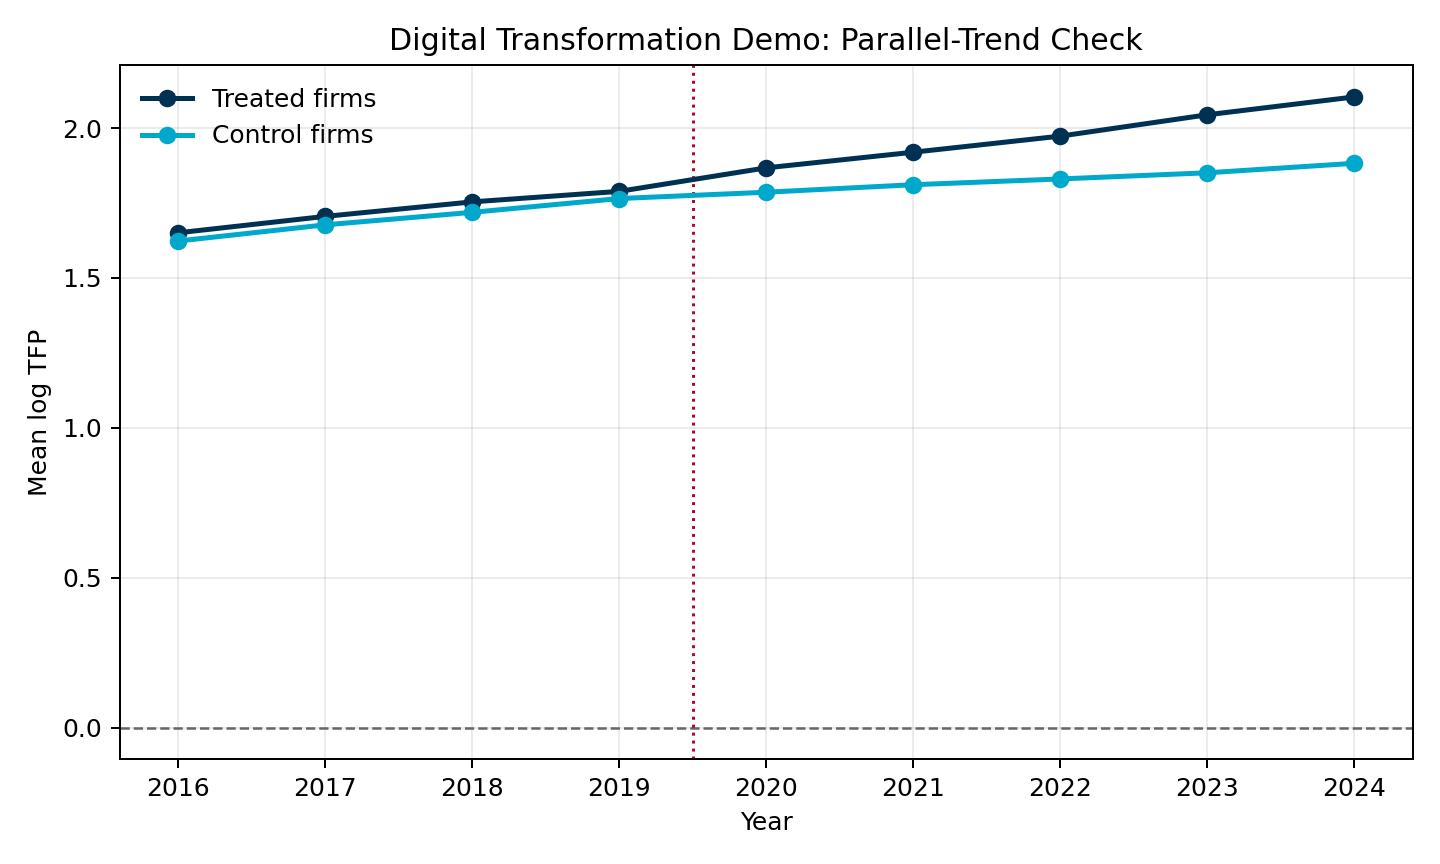
\includegraphics[width=0.78\textwidth]{digital_parallel_trends.png}
\caption{合成企业面板中的平行趋势诊断}
\label{fig:parallel-trends}
\end{figure}

\begin{figure}[htbp]
\centering
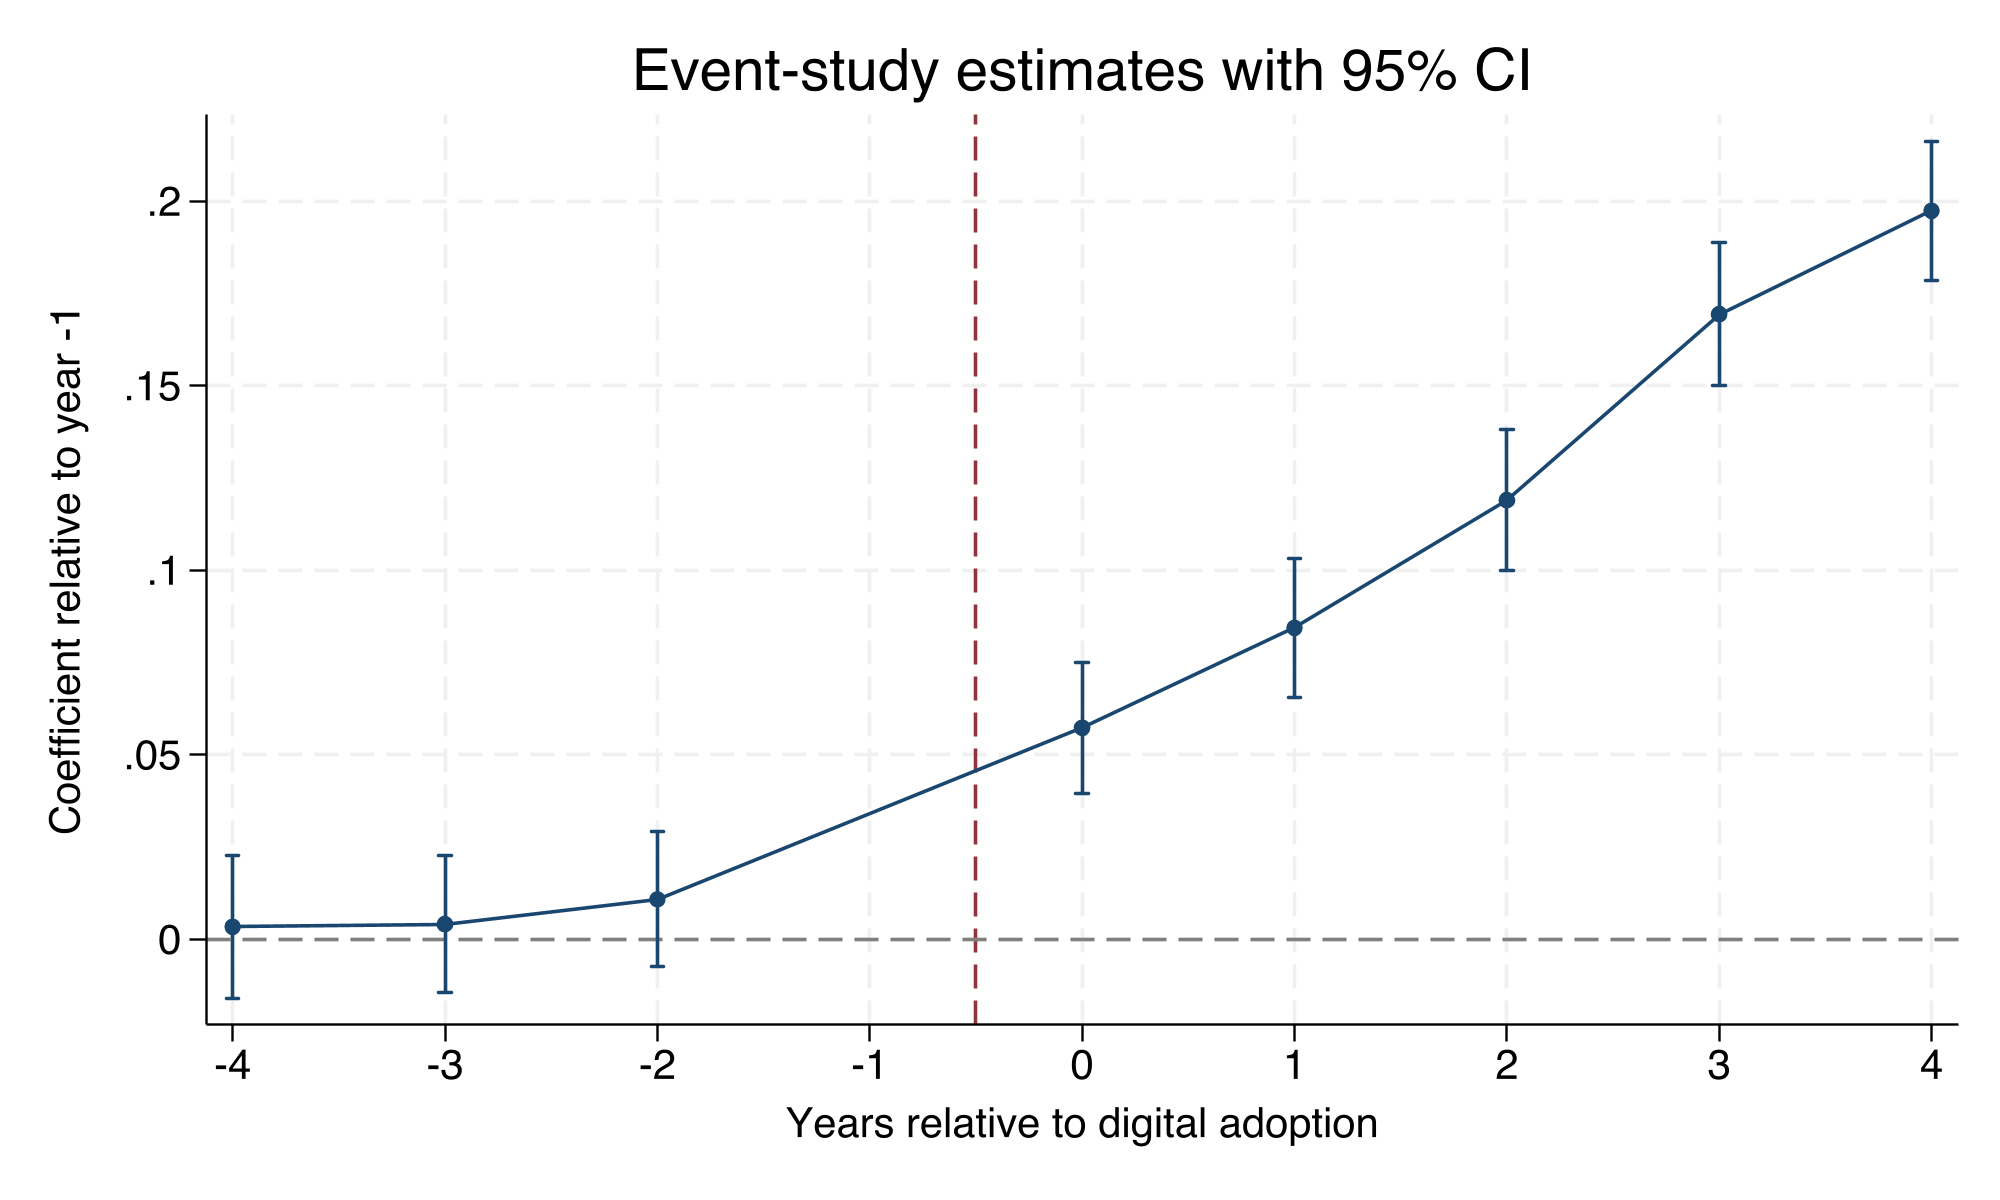
\includegraphics[width=0.78\textwidth]{stata_event_study_ci.png}
\caption{事件研究估计与 95\% 置信区间}
\label{fig:event-study}
\end{figure}

\begin{table}[htbp]
\centering
\caption{事件研究关键系数（基准期：处理前一年）}
\label{tab:event-study}
\begin{tabular}{ccccc}
\toprule
相对年份 & 系数估计 & 标准误 & $t$ 值 & $p$ 值 \\
\midrule
$-4$ & 0.0034 & 0.0099 & 0.34 & 0.733 \\
$-3$ & 0.0041 & 0.0095 & 0.43 & 0.665 \\
$-2$ & 0.0108 & 0.0093 & 1.16 & 0.245 \\
$0$  & 0.0573 & 0.0091 & 6.32 & 0.000 \\
$1$  & 0.0844 & 0.0096 & 8.78 & 0.000 \\
$2$  & 0.1190 & 0.0098 & 12.17 & 0.000 \\
$3$  & 0.1694 & 0.0099 & 17.04 & 0.000 \\
$4$  & 0.1974 & 0.0096 & 20.50 & 0.000 \\
\bottomrule
\end{tabular}
\begin{flushleft}
\footnotesize 注：结果来自 \texttt{output/stata\_event\_study.csv}。
\end{flushleft}
\end{table}

\section{安慰剂检验}

安慰剂检验只使用处理前样本，并假设处理组企业在 2018 年已经受到虚假处理。估计结果见表 \ref{tab:placebo}：\texttt{placebo\_digital\_2018} 的系数约为 0.0015，标准误约为 0.0074，$p$ 值约为 0.835。这说明在合成数据中，处理前没有明显的虚假政策效应。该检验支持工作流中的诊断逻辑，但仍不能替代真实研究中对识别假设的论证。

\begin{table}[htbp]
\centering
\caption{安慰剂检验结果（仅处理前年份样本）}
\label{tab:placebo}
\begin{tabular}{lccccc}
\toprule
变量 & 系数估计 & 标准误 & $t$ 值 & $p$ 值 & 观测值 \\
\midrule
Placebo\_Digital\_2018 & 0.0015 & 0.0074 & 0.21 & 0.835 & 1440 \\
\bottomrule
\end{tabular}
\begin{flushleft}
\footnotesize 注：结果来自 \texttt{output/stata\_placebo\_results.csv}。
\end{flushleft}
\end{table}

\section{理论机制：AI 采用成本收益模型}

Matlab 部分将数字化转型解释为企业 AI 采用决策。企业 $i$ 的管理能力为 $m_i$，选择 AI 使用强度 $x_i \in [0,1]$。采用 AI 的净收益为
\begin{equation}
V_i(x_i) = (\phi + \lambda m_i)x_i - \frac{1}{2}\psi x_i^2 - c_i.
\end{equation}
企业先使用有界优化求解最优强度 $x_i^*$，再根据 $V_i(x_i^*)$ 是否大于零决定是否采用 AI。模型用 Stata DID 估计目标校准参数 $\phi$。校准结果见表 \ref{tab:theory-calibration}，其中 $\phi$ 约为 0.8659，模型平均收益约为 0.1209，AI 采用率约为 0.8197。

\begin{table}[htbp]
\centering
\caption{Matlab 理论模型校准结果}
\label{tab:theory-calibration}
\begin{tabular}{lcc}
\toprule
参数/统计量 & 符号 & 数值 \\
\midrule
目标效应（Stata DID） & Target effect & 0.1209 \\
生产率基准收益参数 & $\phi$ & 0.8659 \\
边际收益参数（管理能力） & $\lambda$ & 0.1200 \\
二次成本参数 & $\psi$ & 1.8000 \\
固定采用成本 & $c_0$ & 0.0600 \\
成本敏感系数 & $\kappa$ & 0.1000 \\
模型平均净收益 & Mean gain & 0.1209 \\
模型收益标准差 & SD gain & 0.0852 \\
AI 采用率 & Adoption share & 0.8197 \\
\bottomrule
\end{tabular}
\begin{flushleft}
\footnotesize 注：结果来自 \texttt{output/matlab\_theory\_estimates.csv}。
\end{flushleft}
\end{table}

图 \ref{fig:theory-model} 展示不同管理能力企业的模型预测生产率收益。管理能力较高的企业因为采用成本相对更低、AI 使用回报更高，更容易采用 AI 并获得更高收益。该模型只是机制展示，不是对真实企业行为的结构估计。

\begin{figure}[htbp]
\centering
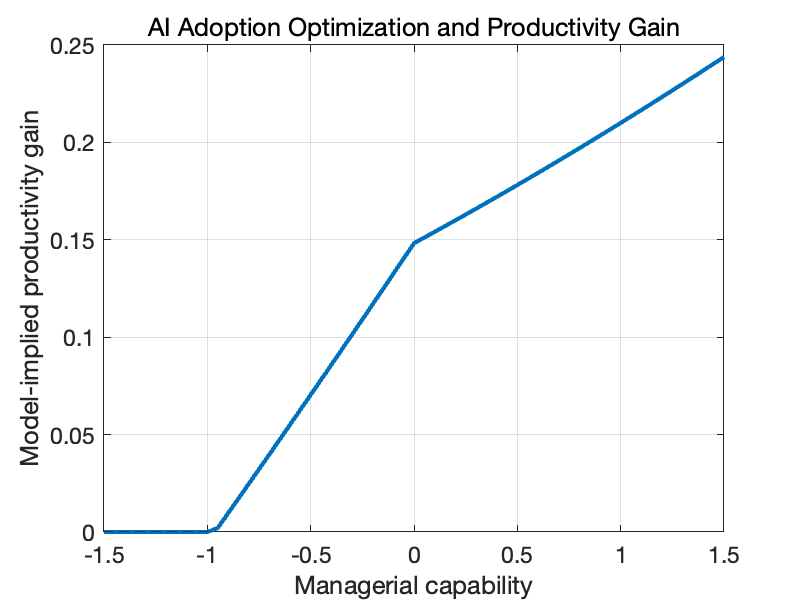
\includegraphics[width=0.78\textwidth]{matlab_theory_model.png}
\caption{AI 采用优化模型中的生产率收益}
\label{fig:theory-model}
\end{figure}

\section{讨论与局限}

本文最大的局限是数据完全由模拟生成。因此，所有估计值只说明工作流从数据生成、Stata 回归、Matlab 机制模拟到论文写作之间是连贯的，不能说明真实企业采用数字技术后一定会提高生产率。第二，事件研究和平行趋势图是诊断工具，不是识别假设的形式证明。第三，理论模型被有意设计得很简洁，只展示成本收益权衡，并未估计真实企业的技术采用结构参数。

\section{结论}

本文展示了一个完整的经济学研究写作工作流。合成数据中的 DID 估计、事件研究、安慰剂检验和 Matlab 机制模型共同构成一个可复现示范。更重要的是，该示范说明 AI 工具可以辅助研究者把可执行分析转化为正式论文文本，但研究者仍必须核查文献、验证代码、检查编译结果，并明确区分演示性结果和真实经验证据。

\section{AI 写作与复现审计附录}

本文写作使用了 AI 辅助工具读取 notebook、输出文件和 LaTeX 初稿，并生成中英文论文草稿。研究者保留了合成数据限制、估计对象、聚类标准误、识别诊断和文献核查要求。所有引用均来自 DOI 或 Crossref 可核查条目；未能核查的文献没有进入参考文献列表。LaTeX 源文件通过 XeLaTeX 编译验证，审计记录见项目根目录下的 \texttt{audit-log.md}。

\bibliographystyle{apalike}
\bibliography{references}

\end{document}